   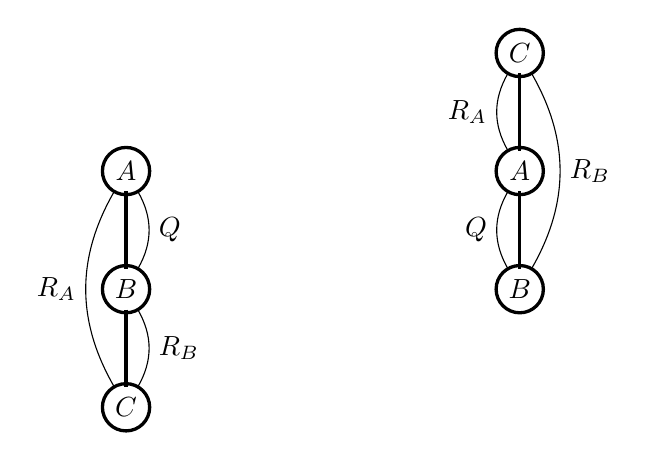
\begin{tikzpicture}[scale=1.0,>=stealth]
%       \draw [help lines] (0,0) grid (10,7);
       
       \draw [very thick] (2,4) circle (0.3)
              node [name=A] {$A$};
       \draw [very thick] (2,2.5) circle (0.3)
              node [name=B] {$B$};
       \draw [very thick] (2,1) circle (0.3)
              node [name=C] {$C$};
       \draw [very thick] (A) -- (B);
       \draw [very thick] (B) -- (C);
       \path (A) edge [bend left] node [right] {$Q$} (B)
             (B) edge [bend left] node [right] {$R_B$} (C)	
             (A) edge [bend right] node [left] {$R_A$} (C);

    \begin{scope}[xshift=5cm]
       \draw [very thick] (2,4) circle (0.3)
              node [name=A] {$A$};
       \draw [very thick] (2,2.5) circle (0.3)
              node [name=B] {$B$};
       \draw [very thick] (2,5.5) circle (0.3)
              node [name=C] {$C$};
       \draw [very thick] (A) -- (B);
       \draw [very thick] (A) -- (C);
       \path (A) edge [bend right] node [left] {$Q$} (B)
             (B) edge [bend right] node [right] {$R_B$} (C)	
             (A) edge [bend left] node [left] {$R_A$} (C);
    \end{scope}

   \end{tikzpicture}
